\section{Optimizations (Ready)}\label{sec:opt}
\name performs many of the standard compiler optimizations,
such as Dead Code Elimination and Constant Propagation.
Some of them, however, play a much more important role for reconfigurable accelerator because they
have a direct impact on resource usage.
Other optimizations can be counter-intuitive, as they introduce redundant computation that
reduces resources without necessarily impacting performance.
In this discussion, we focus our primary objective on performance.
Reducing resources is an indirect objective as resource reduction enable larger parallelization factors,
which in turn improves performance.
Other objectives, such as power saving, is left as future work.

\subsection{Description (Ready)}\label{sec:des}

\begin{figure*}
\centering
\begin{subfigure}[b]{0.4\textwidth}
\inputminted{python}{code/msr.py}
\caption{Input program}
\end{subfigure}
\hfill
\begin{subfigure}[b]{0.5\textwidth}
\inputminted{python}{code/msrctx.py}
\caption{Context graph}
\end{subfigure}
\caption[Memory strength reduction]{
  (a) shows an example where read and write address of \texttt{mem} can be constant folded because
  loop A and loop C are fully parallelized.
  Instead of mapping \texttt{mem} into a scratchpad, which heavily underutilize the capacity of the 
  scratchpad, \name maps the memory into a non-indexable vector stream in (b). The vector stream
  stores address [0-15] of the original memory, whereas the reader $R1$ requests address [15-0] instead.
  \name uses a \texttt{shuffle} operator to swap the vector elements based on reader's expected order.
  This is the same \texttt{shuffle} operator we introduced in the memory partitioning section
  \Cref{sec:memsplit}. 
}
\label{fig:msr}
\end{figure*}

\subparagraph{Memory strength reduction (msr).} Like traditional strength reduction on arithmetics,
\name{} replaces expensive on-chip memories with cheaper memory types whenever possible.
Scratchpad, input buffer, and pipeline register are different types of on-chip memory on Plasticine from
the most expensive to the cheapest.
%We map register accumulation in the program with single-cycle initiation interval to pipeline registers.
For example, \name maps on-chip array to a scratchpad by default. However, if all of the readers and
writers of the array index into memory with constant addresses, often as a result of constant propagation of full
parallelized loops, \name maps the memory to the input buffer of a context, and setup datapath to
connect the reader and writer directly.
\Cref{fig:msr} shows an example of strength reduce a scratchpad into an input buffer with additional
operations.
Fully parallelized loops are a common outcome of an automatic design space exploration of the parallelization factors.
We also use it as a way for the user to explicitly program vectorized streaming operation for
Plasticine.

\begin{figure*}
\centering
\begin{subfigure}[b]{0.45\textwidth}
\inputminted{python}{code/rteg1.py}
\caption{Example with variable}
\end{subfigure}
\hfill
\begin{subfigure}[b]{0.45\textwidth}
\inputminted{python}{code/rteg2.py}
\caption{Example with queue}
\end{subfigure}
\caption[Examples of route through elimination]{
  (a) and (b) shows route through opportunities in the program.
  These opportunities are often outcome of lowering and other optimizations. To proof the route
  through is safe, \name needs to have access to all readers and writers of a memory, and analyze
  the control structure around the memory accesses.
  In addition to saving on the memory, the optimization eliminates the basic block in line 7 of (a)
  and line 8 of (b), which saves a context.
}
\label{fig:rtelm}
\end{figure*}

\subparagraph{Route-Through Elimination (rtelm).} 
For patterns where the content of a non-indexable memory (M1) is read and written to another memory
(M2), \name{} eliminates the intermediate access and feeds the output of M1's writer (W1) directly to M2's
reader (R2) if it can prove the propagation is safe.
\Cref{fig:rtelm} shows examples of route-through opportunities.
These patterns are often the
outcome of multiple levels of compiler lowering and the \emph{msr} optimization. 
Eliminating route-through patterns can simplify control hierarchy and reduce the number of basic blocks, which eliminates contexts.

\begin{figure*}
\centering
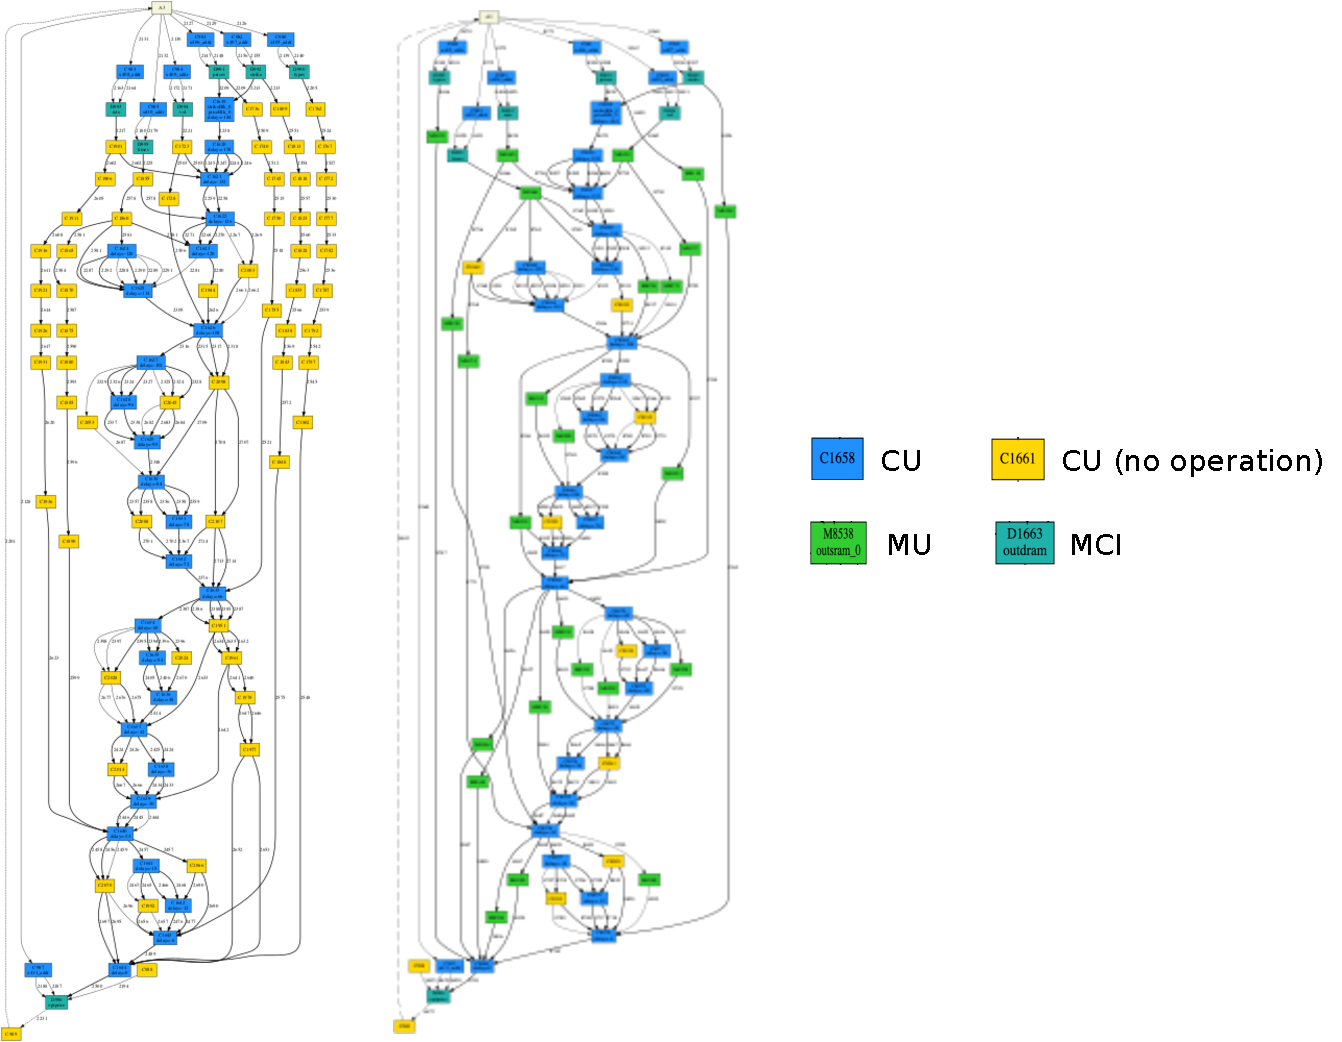
\includegraphics[width=0.8\textwidth]{figs/retiming.pdf}
\caption[Retiming]{
  Virtual unit dataflow graph (VUDFG) after retiming. CU: virtual compute unit. MU: virtual memory
  unit. MCI: memory controller interface.
  Left: retiming with input buffer only. Right: retiming with either input buffer or scratchpad.
  The yellow CUs are CUs used for retiming. The original program does not have MU and the yellow MU
  on the right are MUs used for retiming. 
}
\label{fig:retiming}
\end{figure*}
\subparagraph{Retiming with scratchpad (retime-mem).} 
By default, \name{} uses input buffers in PU for retiming purposes. 
This option enables \name{} to use scratchpad memory to retime paths requiring deep buffers.
\Cref{fig:retiming} shows VUDFGs after retiming with and without scratchpad retiming. As we can see,
allowing scratchpad and input buffer for retiming significantly reduces the total number of retiming
units.

\subparagraph{Crossbar datapath elimination (xbar-elm).}
Although in the general cases described in \Cref{sec:memsplit}, 
crossbar data paths between accessors and memory partitions are very expensive, 
the BA can often be statically resolved to a constant vector for certain
parallelization factors and address patterns.  
When BA is a constant, \name{} can use this information to intelligently 
group banks into memory partitions that reduce the crossbar to a partial 
or a point-to-point connection.
This is an important optimization that prevents resource scaling quadratically with increasing
parallelization in the common cases.

\begin{figure*}
\centering
\begin{subfigure}[b]{0.6\textwidth}
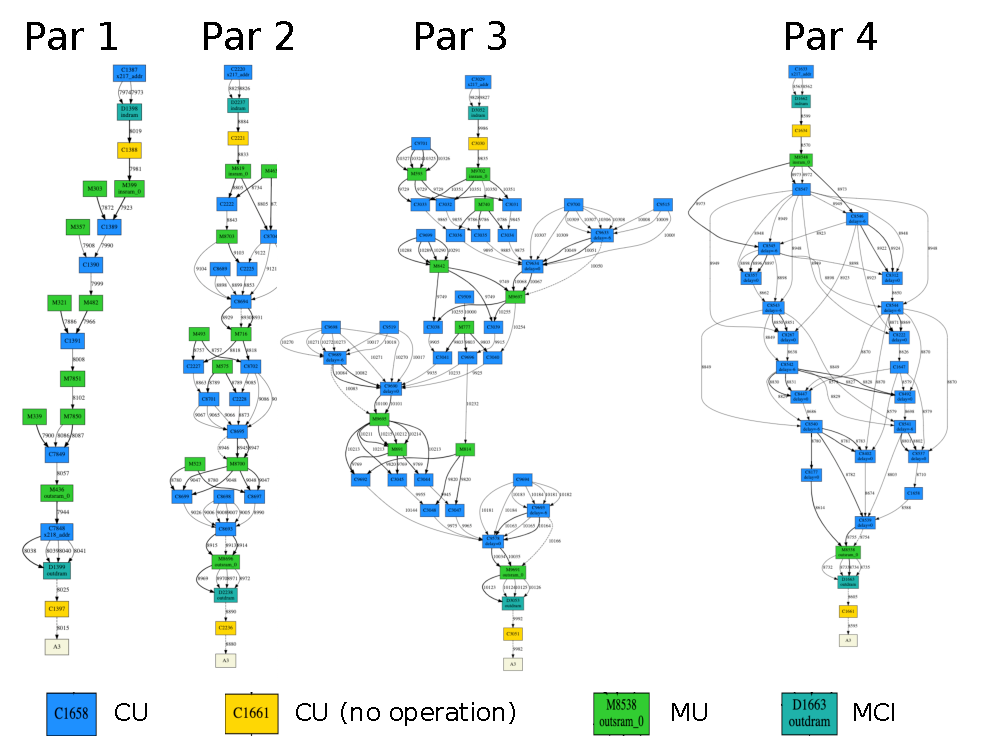
\includegraphics[width=1\textwidth]{figs/mlpunroll.pdf}
\caption{VUDFGs with different parallelization factors}
\end{subfigure}
\hfill
\begin{subfigure}[b]{0.39\textwidth}
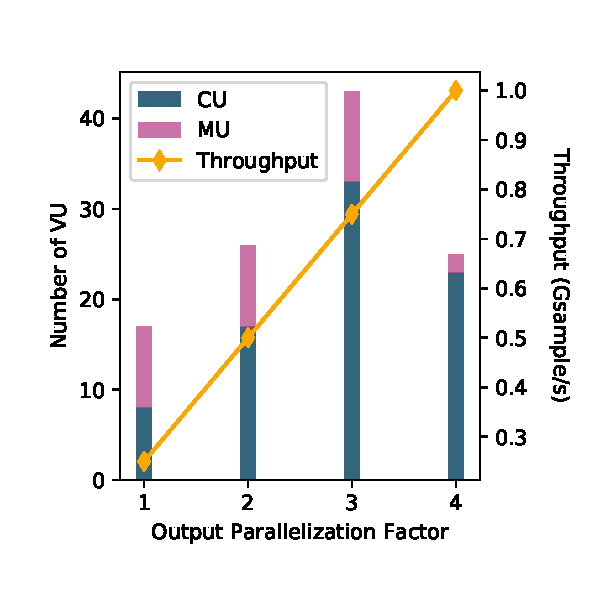
\includegraphics[width=1\textwidth]{figs/mlp.pdf}
\caption{Throughput and resource as a function of parallelization factor}
\end{subfigure}
\caption[MLP case study]{
  A 4x4x4 MLP case study. 
  Light-weight models like this can be useful in ultra high-bandwidth and
  low-latency inference in packet processing~\cite{taurus}.
  (a) shows changes in VUDFG as we parallelize the output dimension.
  The input dimension of MLP is vectorized across SIMD lanes.
  As reaching par factor at 4, the intermediate memory in MU gets optimized away due to constant
  folding and rtelm on fully unrolled loops. (b) shows the throughput and resource increase as the
  output dimension is parallelized.
}
\label{fig:mlp}
\end{figure*}

Combined with \emph{msr} and \emph{rtelm} mentioned above, \name is able to 
dramatically reduce the resource usage for certain parallelization factors.
\Cref{fig:mlp} shows an interesting case study on an MLP presenting performance scaling and resource
increase while scaling up parallelism.
\Cref{fig:mlp} (b) demonstrates that Plasticine can have resource
non-linearly increasing with parallelization factors, while having perfect performance scaling, due to compiler optimizations.

\subparagraph{Read address duplication (dupra).} 
%The long traveling path for BA from the address context to the receiver context showing in memory partitioning
%\Cref{sec:memsplit} \Cref{fig:memsplit} can cause pipeline stalls due to the imbalance datapath between
%the BA forwarding path and the memory data path.
Between the address context and receiver contexts in memory partitioning shown in \Cref{sec:memsplit}
\Cref{fig:memsplit},
the imbalance datapaths between BA forwarding and request datapath can cause significant pipeline
stalls, limiting the overall application performance to a small fraction of the ideal throughput.
When parallelizing the memory access, the OR tree in the merge context gets partitioned into a tree
of contexts, which further increases the mismatch in latency between the imbalanced datapaths.
Instead of retiming BA forwarding path, 
this compiler flag forces \name to duplicate the BA computation using local states
within the receiver context, which could use fewer resources than retiming.

\subparagraph{Global Merging (merge).}
After all VUs satisfy the hardware constraint, we perform a global optimization to compact small VUs into larger VUs. 
Merging has a very similar problem statement as compute partitioning (\Cref{sec:compsplit}) except with more constraints.
For merging, the VUDFG is the graph, the VUs are the nodes, and the merged VUs are partitions.
Unlike the partitioning problem, which uses a single set of cost metrics to determine if a partition
is valid, the merged partition
can be mapped to any PU available on-chip, each having a different set of cost metrics and a
quantity limit.
%The traversal-based algorithm requires a reference cost from PU to check if the merged VU still satisfies the hardware constraint.
When adding a new VU \emph{m} to a partition \emph{P} in the traversal-based algorithm, 
we first take the union of the domains of VUs within the current partition, and
intersect with the domain of \emph{m}.
The domain of the merged partition \emph{M} is updated to all PUs within this intersection that \emph{M} can fit.
\begin{align}
  M &= P \cup \{m\} \\
  dom(M) &= \{ p | p \in \{\cup\ dom(n)\ |\ \forall n \in P\} \cap dom(m), cost(M) \leq cost(p) \}
\end{align}
The caveat is that even if \emph{M} has non-empty domain, the bipartite graph might not have a possible 
assignment after merging, as \emph{M} might fit in a larger PU with insufficient quantity.
Therefore, we perform the feasibility checking of the bipartite assignment at each step
of merging, shown in \Cref{algo:check}, and only merge if the assignment is feasible.

The solver-based solution combines the VU merging with VU to PU assignment as a joint problem. 
The output of merging gives both partition assignment as well as a PU type assignment, which
eliminates the risk of infeasible assignment due to merging in the traversal-based solution.

\subparagraph{Reversed Loop Invariant Hoisting}

\begin{figure*}
\centering
\hfill
\begin{subfigure}[b]{0.4\textwidth}
\inputminted{python}{code/hoisting.py}
\caption{Input program}
\end{subfigure}
\hfill
\begin{subfigure}[b]{0.4\textwidth}
\inputminted{python}{code/reversehoisting.py}
\caption{Reversed loop invariant hoisting}
\end{subfigure}
\hfill
\caption[Reversed loop invariant hoisting]{
  The original program requires at least two contexts to execute Block 1 and Block 2.
  By moving the invariant instruction \texttt{c = a + b} into the loop body, (b) only needs a single
  context instead. Because instructions within \texttt{Block 2} are pipelined across loop
  iterations, adding instructions in the loop body introduce minimum performance impact.
  This transformation is beneficial until \texttt{Block 2} exceeds six operations, at which point
  both version consume the same amount of resources.
}
\label{fig:reversehoisting}
\end{figure*}

A common loop optimization on traditional CPU is to move loop-invariant expressions 
outside of the loop body to reduce computation. 
This transformation, however, can introduce more basic blocks in the program, that translates to
more contexts on Plasticine.
Therefore, the reversed loop invariant hoisting, which moves loop-invariant expressions into the loop body, can sometimes save resources by simplifying the control structure, as shown in 
\Cref{fig:reversehoisting}.
Because instructions within the basic blocks are pipelined, 
moving instructions into the loop body increases computation without hurting throughput, which
dominant the performance for spatial architecture.
Currently, we rely on the user to perform this optimization manually.

\subsection{Evaluation (WIP)}

\begin{figure*}
\centering
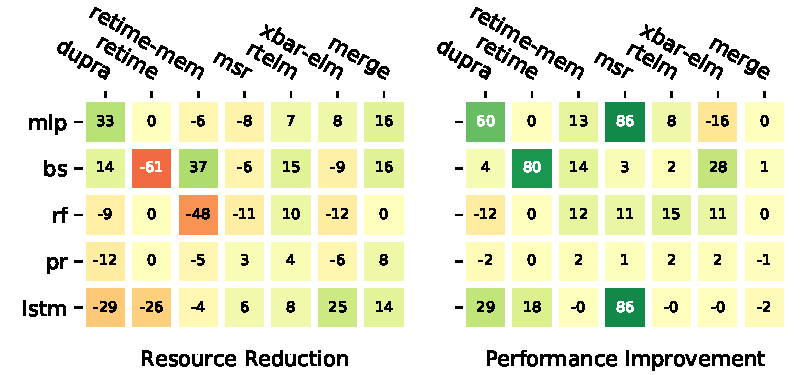
\includegraphics[width=0.8\textwidth]{figs/heat.pdf}
\caption[Optimization effectiveness]{
  Optimization effectiveness. Percentage resource reduction or performance improvement from each
  optimization. The heat map shows the maximum differences when turning on/off the optimization, 
  while fixing other optimizations at the most optimum combination for the application.
  Each application has a large design space with various parallelization factors in different loops, 
  we report a design point that has the maximum impact, either positively or negatively.
}
\label{fig:heat}
\end{figure*}

\Cref{fig:heat} presents the evaluation of performance improvement and resource reduction from
optimizations discussed in \Cref{sec:des}.

\emph{merge} and \emph{rtelm} are optimizations that gives a consistent resource improvement for most applications.
\emph{dupra} and \emph{msr} helps \emph{\bf mlp} and \emph{\bf lstm}, which are heavily partitioned during the memory-partitioning stage.

\emph{dupra} significantly reduces unbalancing in the data path caused due to the large merge tree generated by memory partitioning.
\emph{retime} can have a significant impact on the performance of the application at the cost of an increase in resource usage.
Using scratchpad as a retiming buffer with the \emph{retime-mem} flag can significantly reduce resource usage.

